% !TEX root = ../../../I4PRJ, Grp3 - Rapport.tex
\subsection{iOS}
Til iOS er der udviklet et view-lag med UIKit og C\#. Det findes under namespace "Smartpool.Application.iOS."

\subsubsection{Design}
I iOS applikationen designes view-klasser, der implementerer view-interfacet defineret i præsentationslaget. Brugergrænseflader på iOS platformen designes med frameworket UIKit, hvor hvert view en tilhørende controller-klasse. iOS designet tager højde for dette, ved at bruge UIKits controller-klasse som en bro, i mellem Smartpools præsentationslag, og UIKits view-lag. Designet er derfor lavet således, at controller-klasserne på iOS implementerer view-interfacet fra præsentationslaget.

SignUpViewBridge og StatViewBridge er de to klasser i iOS-applikationen, som implementerer hhv. ISignUpView og IStatView. Udover at implementere view-interfacet, indeholder begge klasser user interface elementer fra UIKit frameworket. SignUpViewBridge-klassen er klassen designet til at indeholde en række tekstfelter, og en knap til at fuldende brugeroprettelsen. SignUpViewBridge nedarver i UIKit konteksten, fra UIViewController-klassen. StatViewBridge nedarver fra UITableViewController, der kan opsættes til at præsentere en dynamisk liste. StatViewBridge indeholder en UIBarButtonItem, der kan bruges til at skifte imellem pools i systemet. Deres design fremgår af figur~\ref{fig:ios_viewbridges}.

\begin{figure}
	\centering
	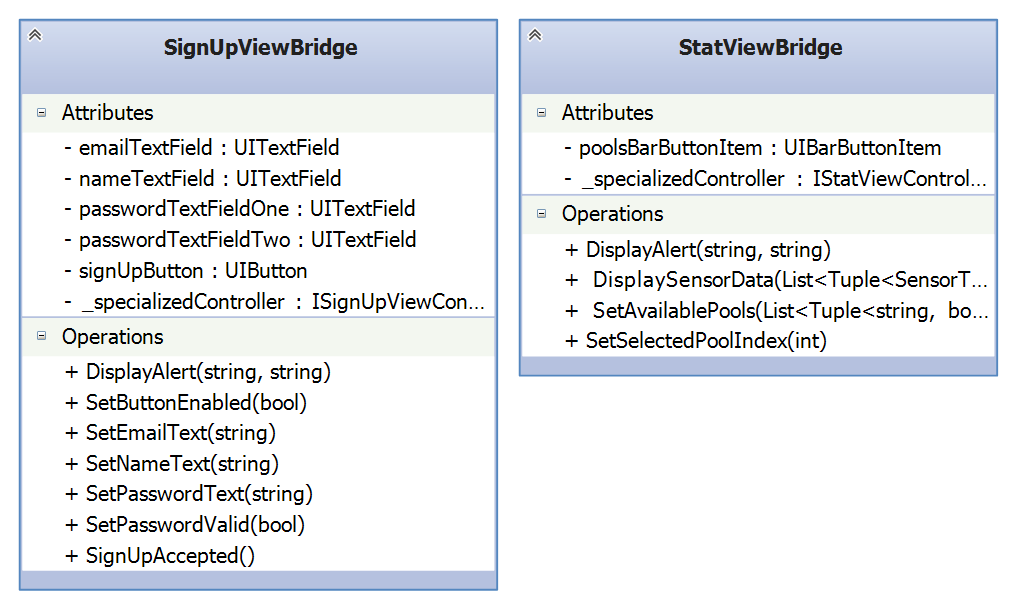
\includegraphics[width=0.7\linewidth]{figs/design/ios_viewbridges}
	\caption{SignUpViewBridge og StatViewBridge}
	\label{fig:ios_viewbridges}
\end{figure}

For yderligere forklaring se dokumentation afsnit Applikationslaget under Design.